% !TEX encoding = UTF-8 Unicode
%!TEX root = thesis.tex
% !TEX spellcheck = en-US
%%=========================================
\chapter{Results}

The results will be introduced in the same order as the experiments were conducted. First, the results of matching of one of the EDX datasets with the SPED dataset will be presented. This is followed the position matching of the various EDX datasets with the overview images. Lastly, the calculated $\zeta$-factors and the quantification of the samples using the $\zeta$-factor method and the Cliff-Lorimer technique are displayed.

\section{Dataset matching}

\cref{fig:edx-in-sped} shows the results of matching the largest EDX dataset with the SPED dataset. As explained in \cref{sec:method/dataset matching}, these images have been processed to be made more similar. \cref{fig:edx-in-sped-edx} shows the EDX image and \cref{fig:edx-in-sped-rectangle} shows the SPED image with a rectangle indicating where the best fit of the EDX image was found. 

\begin{figure}
\begin{subfigure}{.5\textwidth}
	\centering
	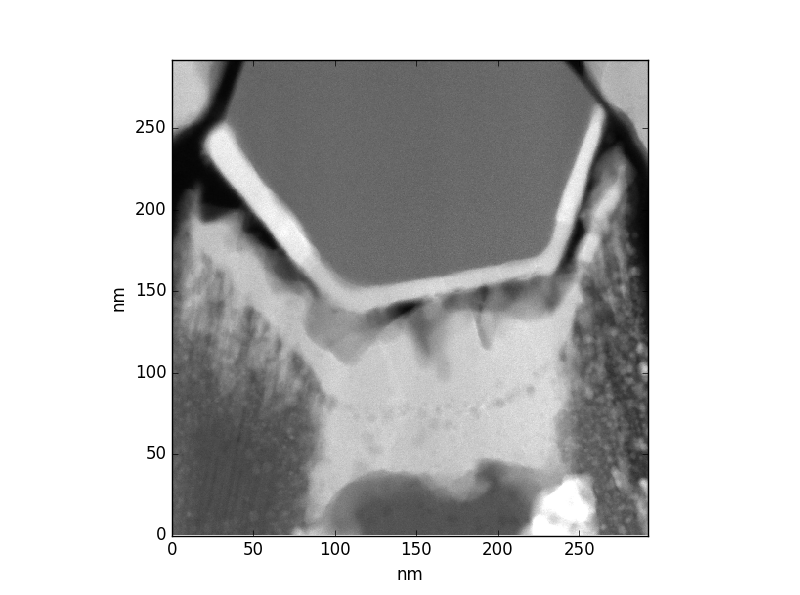
\includegraphics[width=\linewidth]{fig/in-rectange}
	\caption{++++++}
	\label{fig:edx-in-sped-edx}
\end{subfigure}%
\begin{subfigure}{.5\textwidth}
	\centering
	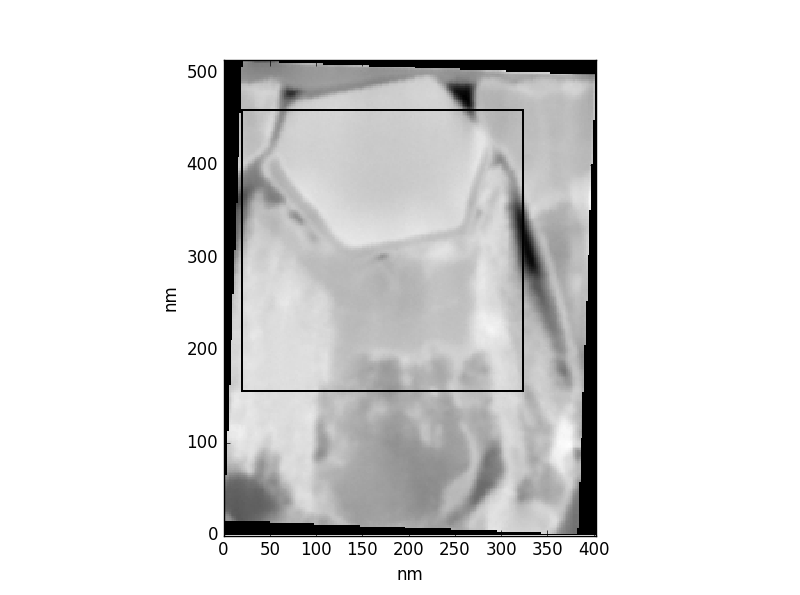
\includegraphics[width=\linewidth]{fig/sdrot-with-rectange}
	\caption{++++++}
	\label{fig:edx-in-sped-rectangle}
\end{subfigure}
\caption{plots of....}
\label{fig:edx-in-sped}
\end{figure}

%As the correct result is unknown, it is difficult to quantify the error in the fit. An attempt was made by looking at the difference between the matching value for the best position, shown in \cref{fig:edx-in-sped-rectangle}, and the higher values. The matching values are defined in \cref{eq:matching value}. \cref{fig:edx-sped-rectangle-match-graph} shows the relative error of the 100 best matching values with respect to the best match. 

\begin{figure}
	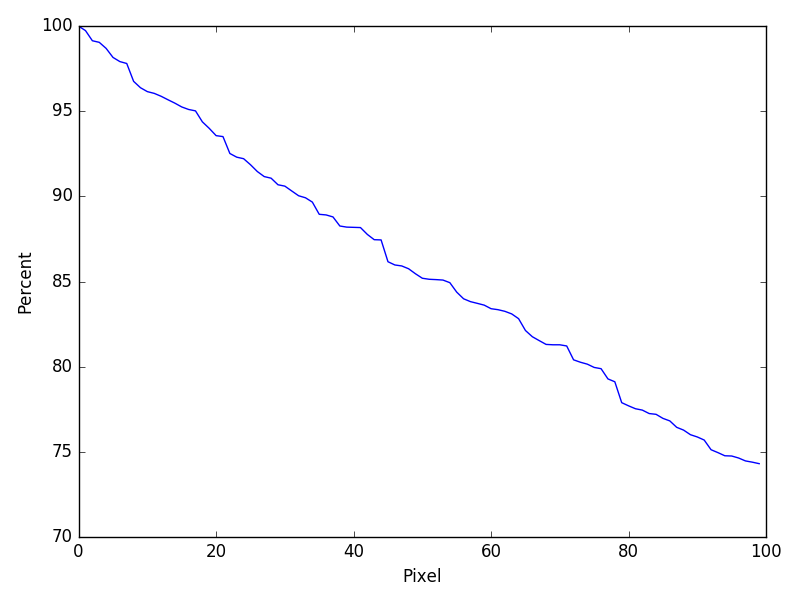
\includegraphics[width=0.7\linewidth]{fig/edx-sped-rectangle-match-graph.png}
	\caption{++++++}
	\label{fig:edx-sped-rectangle-match-graph}
\end{figure}

The results from locating the EDX datasets in the HAADF overview images are displayed in \cref{fig:nonheated-images-in-overview, fig:heated-images-in-overview} for the non-treated and the heat-treated samples, respectively. In the non-treated sample, the two datasets B and D were not correctly located in the overview image. The calculated location of dataset B was completely off, while the position of D was just slightly offset. The actual positions of these datasets were estimated by eye and marked in \cref{fig:nonheated-images-in-overview} as blue dotted rectangles. The rest of the datasets were located correctly, and their positions are shown as red rectangles. For the heat-treated sample, all the datasets that were included in the overview image were correctly located. However, the areas covered by two the datasets A and B were found to not be included in the overview image.

\begin{figure}
	\begin{subfigure}{.5\textwidth}
		\centering
		\includegraphics[width=\linewidth]{"fig/nonheated-images-in-overview (correct)3"}
		\caption{}
		\label{fig:nonheated-images-in-overview}
	\end{subfigure}%
	\begin{subfigure}{.5\textwidth}
		\centering
		\includegraphics[width=\linewidth]{"fig/nonheated-matching-values"}
		\caption{}
		\label{fig:nonheated-matching-values}
	\end{subfigure}
\end{figure}

\begin{figure}
	\begin{subfigure}{.5\textwidth}
		\centering
		\includegraphics[width=\linewidth]{"fig/heated-images-in-overview-ink2"}
		\caption{}
		\label{fig:heated-images-in-overview}
	\end{subfigure}%
	\begin{subfigure}{.5\textwidth}
		\centering
		\includegraphics[width=\linewidth]{"fig/heated-matching-values"}
		\caption{}
		\label{fig:heated-matching-values}
	\end{subfigure}
\end{figure}

The accuracy of the matching for the different datasets are shown in \cref{fig:nonheated-matching-values} for the non-heated sample, and in \cref{fig:heated-matching-values} for the heated values. The horizontal axis shows the different datasets while the vertical axis is the matching value in percent, where $\SI{100}{\percent}$ is defined to be the matching value of the dataset covering the biggest area in each respective sample. The matching of this dataset is assumed to be the most trustworthy due to there being fewer potential locations that resemble the actual location, as there are several distinct features. For the smaller datasets, or more accurately, the datasets with smaller survey images, there might be several different locations in the overview image that all give a fairly good match.

In both figures, the red star is the value of the dataset used as reference, the red circles are the correctly matched datasets while the blue squares are the datasets that resulted in a wrong location. The non-heated sample (\cref{fig:nonheated-matching-values}) shows high values for all the correctly located datasets, and significantly lower values for the wrongly located ones. In addition, it must be noted that the exact location of dataset F was impossible to verify visually due to the survey image not being large enough to distinguish specific features. In the heated sample (\cref{fig:heated-matching-values}), all the red correctly located datasets have high values while the datasets that were not present in the reference image have distinguishably lower values.

\section{Determination of $\zeta$-values}

The calculated $\zeta$-values for all the elements present in the sample are presented in \cref{tab:non-heated zeta-values}, along with which dataset was used to calculate them. All datasets are from the unheated sample except for C*, which is from the heated one.

\begin{table}
	\caption{...}
	\begin{center}
	\begin{tabular}{ccc}

	Element & Dataset & $\zeta$\\ 
	\midrule
	\hline
	Ga & C* & 582\\
	Ga & A  & 608\\
	As & C* & 689\\
	As & A  & 706\\
	GeK & B  & 732\\
	GeK & D  & 741\\
	GeK & A  & 748\\
	GeL & A & 933\\
	GeL & D & 900\\
	GeL & B & 900\\
	Pd & E  & 1248\\
	Pd & A  & 1284\\
	Pd & B  & 1318\\
%	AuL & B  & 3450\\ 
%	AuL & C  & 3473\\
	Au & B & 2397\\
	AuM & C & 2387\\
	\hline
	\end{tabular} 
	\end{center}
	\label{tab:non-heated zeta-values}
\end{table}

These values have been 


\section{Quantification}

\cref{fig:zeta_area1,fig:zeta_area2} shows the compositions of two areas (\cref{fig:zeta_area1_overview,fig:zeta_area2_overview} shows the locations of these areas) in the untreated sample, as calculated using the Cliff-Lorimer ratio method (CL method) and the $\zeta$-factor method with and without absorption correction. All the spectra have been averaged in the horizontal direction. The results are as expected. \cref{fig:zeta_area1_ga,fig:zeta_area1_as} shows that the nanowire consists of Ga and As in a 50/50 ratio, and \cref{fig:zeta_area1_ge,fig:zeta_area1_pd} shows that the next two layers are approximately 100\% Pd and Ge. In the second area, \cref{fig:zeta_area2_pd,fig:zeta_area2_ge,fig:zeta_area2_au} shows that the composition of elements are approximately 100\% Au in the top region, 100\% Pd in the middle and 100\% Ge in the lower region.

All three techniques give fairly similar answers for Ga and As, while the difference between the CL- and $\zeta$-factor methods is significantly higher for Pd, Ge and Au. The inclusion of absorption correction does not give significantly different results for any of the elements, except for the Ge-region in the second area where the absorption correction appears to significantly amplify two peaks. \cref{fig:zeta_area1_all,fig:zeta_area2_all} shows the compositions of all the element as calculated using the $\zeta$-method with absorption correction. There is a clear transitioning length between each of the elements layers where the spectra shows characteristic peaks belonging to both elements. This length is shortest for the transition between GaAs and Pd, and longest between Pd and Ge.

\begin{figure}
	\begin{subfigure}{.5\textwidth}
		\centering
		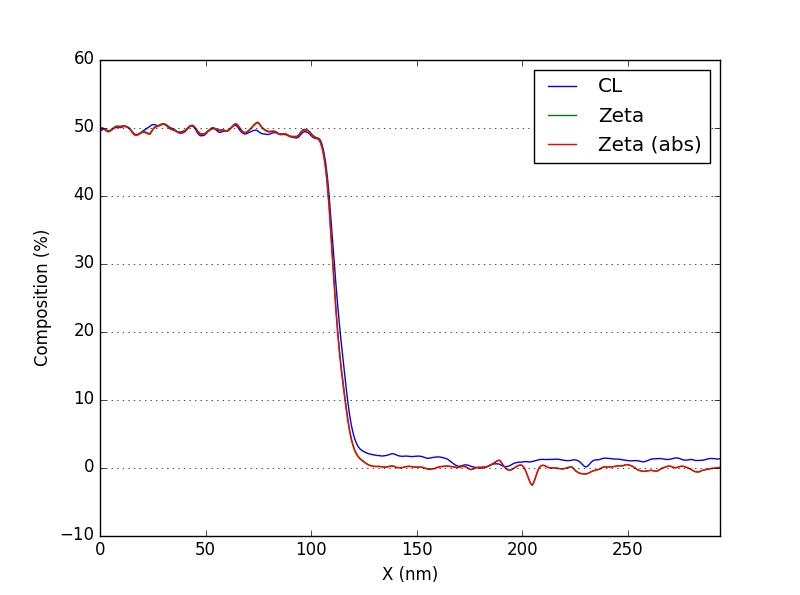
\includegraphics[width=\linewidth]{fig/q/1_ga_nm}
		\caption{}
		\label{fig:zeta_area1_ga}
	\end{subfigure}%
	\begin{subfigure}{.5\textwidth}
		\centering
		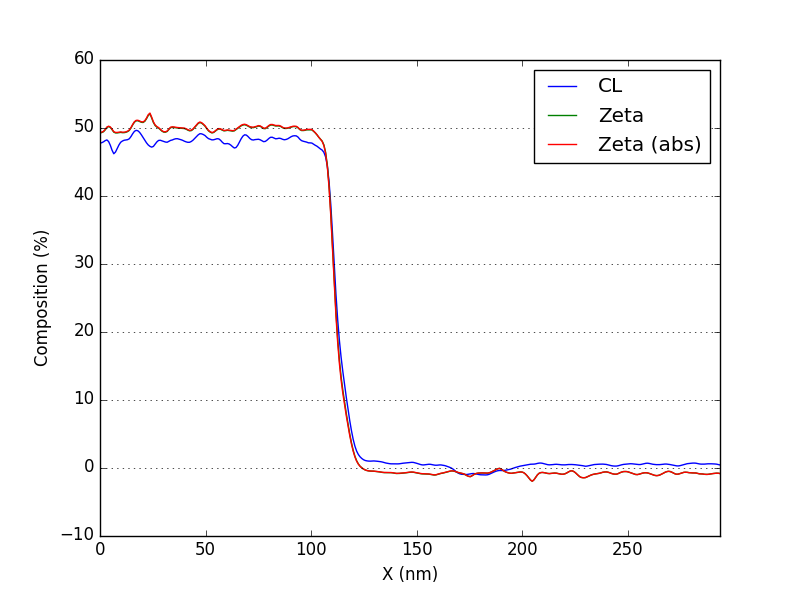
\includegraphics[width=\linewidth]{fig/q/1_as_nm}
		\caption{}
		\label{fig:zeta_area1_as}
	\end{subfigure}
		\begin{subfigure}{.5\textwidth}
			\centering
			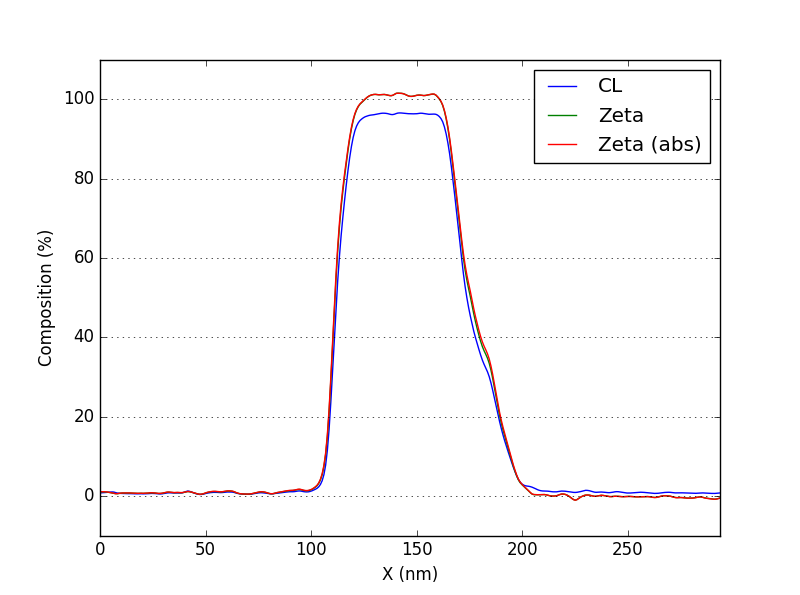
\includegraphics[width=\linewidth]{fig/q/1_pd_nm}
			\caption{}
			\label{fig:zeta_area1_pd}
		\end{subfigure}%
		\begin{subfigure}{.5\textwidth}
			\centering
			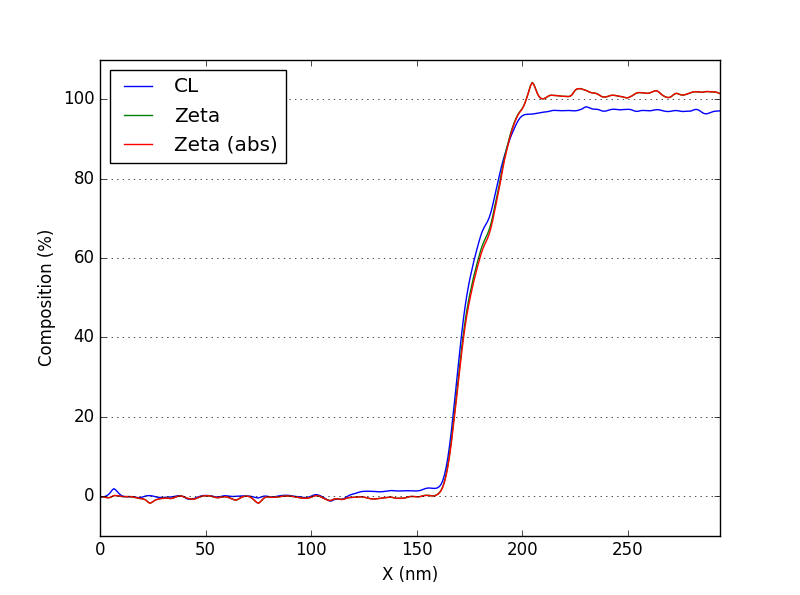
\includegraphics[width=\linewidth]{fig/q/1_ge_nm}
			\caption{}
			\label{fig:zeta_area1_ge}
	\end{subfigure}
		\begin{subfigure}{.5\textwidth}
			\centering
			\includegraphics[width=\linewidth]{fig/q/1_all-abscorr4}
			\caption{}
			\label{fig:zeta_area1_all}
	\end{subfigure}%
	\begin{subfigure}{.5\textwidth}
		\centering
		\newlength\imageheight
		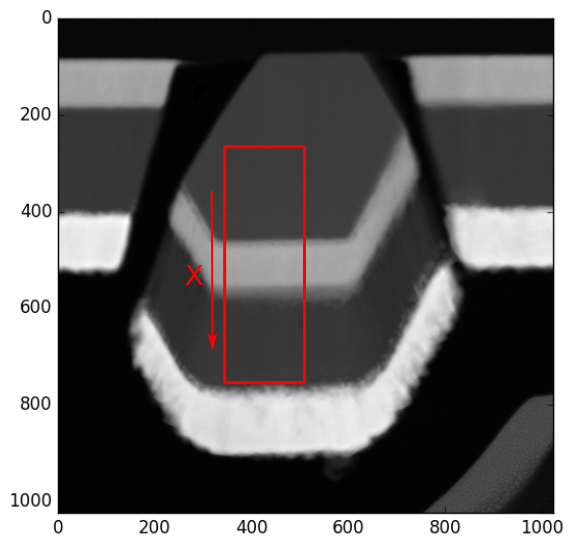
\includegraphics[width=.68\linewidth]{fig/q/1_overview3}
		\caption{}
		\label{fig:zeta_area1_overview}
	\end{subfigure}
	\caption{plots of....}
	\label{fig:zeta_area1}
\end{figure}

\begin{figure}
	\begin{subfigure}{.5\textwidth}
		\centering
		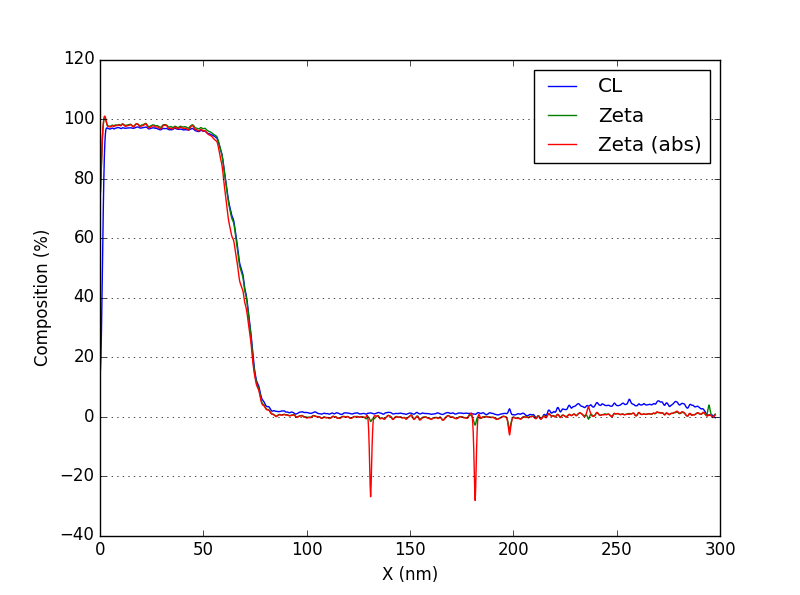
\includegraphics[width=\linewidth]{fig/q/2_pd_nm_GeL}
		\caption{}
		\label{fig:zeta_area2_pd}
	\end{subfigure}%
	\begin{subfigure}{.5\textwidth}
		\centering
		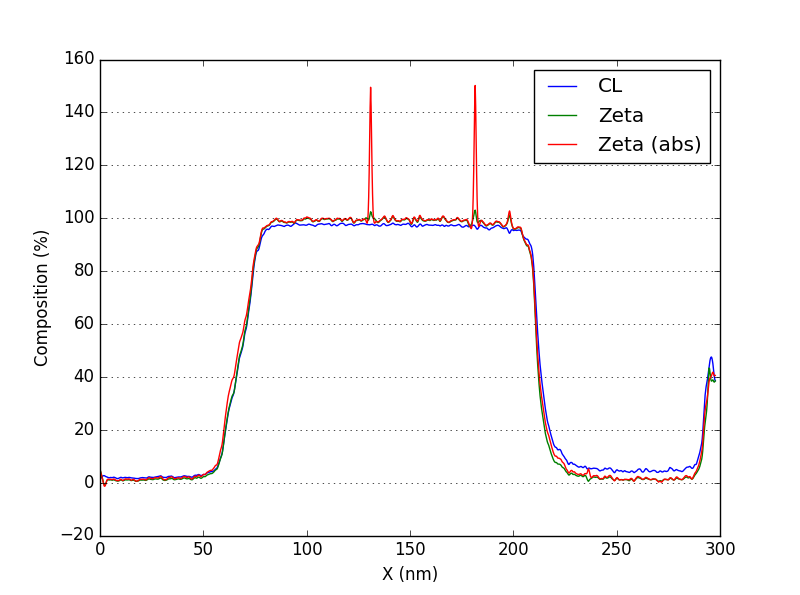
\includegraphics[width=\linewidth]{fig/q/2_ge_nm_GeL}
		\caption{}
		\label{fig:zeta_area2_ge}
	\end{subfigure}
	\begin{subfigure}{.5\textwidth}
		\centering
		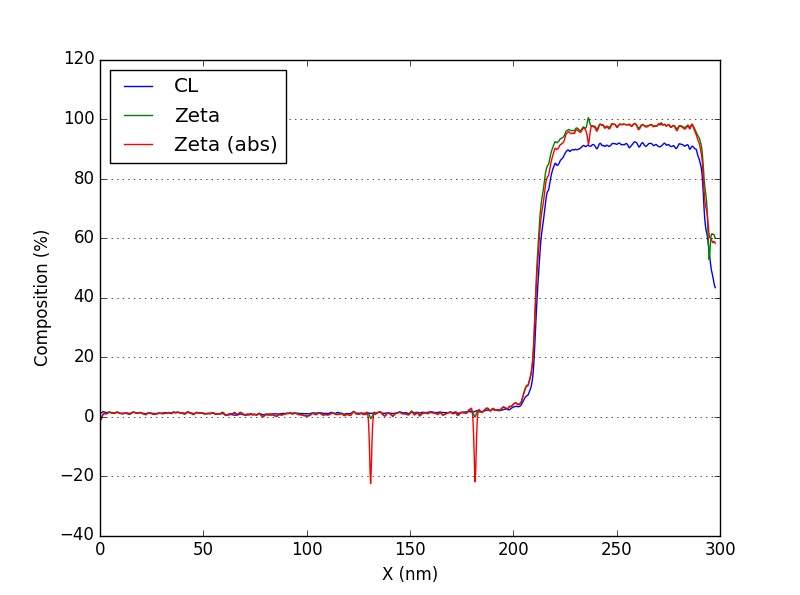
\includegraphics[width=\linewidth]{fig/q/2_au_nm_GeL}
		\caption{++++++}
		\label{fig:zeta_area2_au}
	\end{subfigure}%
	\begin{subfigure}{.5\textwidth}
		\centering
		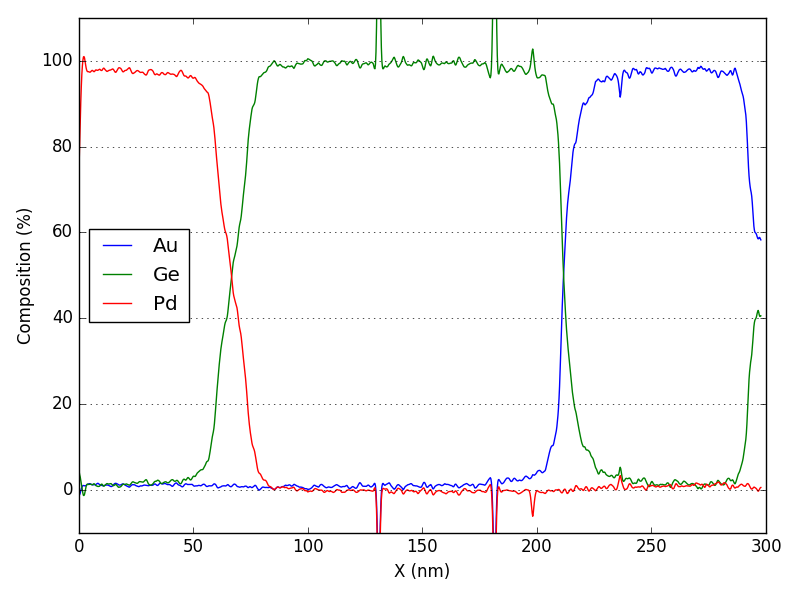
\includegraphics[width=\linewidth]{fig/q/2_all_abscorr_GeL}
		\caption{++++++}
		\label{fig:zeta_area2_all}
	\end{subfigure}
		\centering
	\begin{subfigure}{.5\textwidth}
		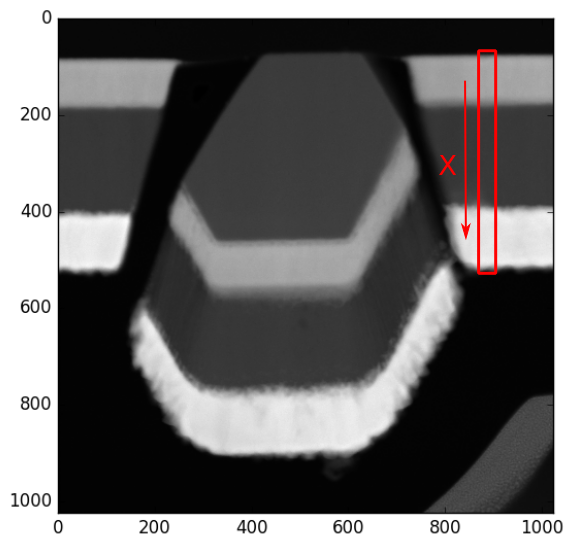
\includegraphics[width=\linewidth]{fig/q/2_overview}s
		\caption{++++++}
		\label{fig:zeta_area2_overview}
	\end{subfigure}
	\caption{plots of....}
	\label{fig:zeta_area2}
\end{figure}

The resulting compositions from areas D and E in the heat-treated sample, using the $\zeta$-factor method with absorption correction, are shown in \cref{fig:D,fig:E} (++++ see Appendix X for equivalent maps from the CL-method and the $\zeta$-method without absorption correction). The areas D and E are located, as seen in \cref{fig:heated-images-in-overview}, in the melted region on the left and right side of the nanowire, respectively. The quantification was done with the assumption that the regions only contained Ga, As, Pd and/or Ge, because the inclusion of Au introduced errors, as explained above (+++ explain this above). The maps have been binned by a factor of two in the x- and y-directions, in order to reduce the effect of outliers.

The upper right region in \cref{fig:Das,fig:Dga}, which is the edge of the nanowire, consists of roughly 35-45\% Ga and 35-45\% As, with the remaining 10-35\% being Ge. 

\begin{figure}
	\centering
	\begin{subfigure}{0.45\textwidth}
		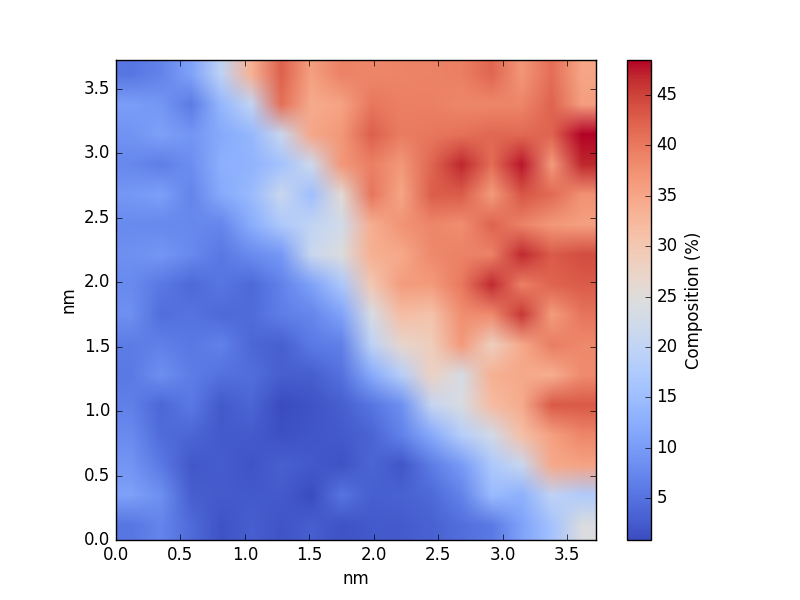
\includegraphics[width=\textwidth]{fig/q/D_heated/_binned_As_zetaAbs}
		\caption{}
		\label{fig:Das}
	\end{subfigure}%
	\hfill
	\begin{subfigure}{0.45\textwidth}
		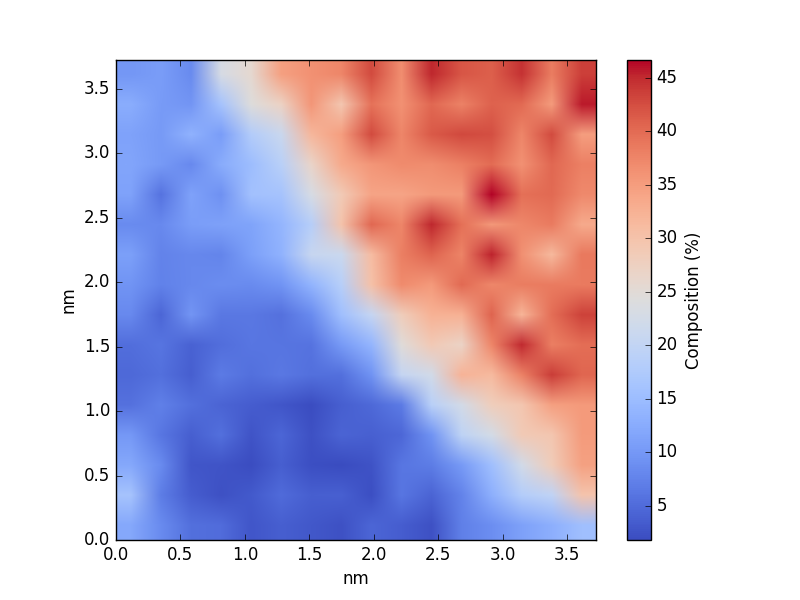
\includegraphics[width=\textwidth]{fig/q/D_heated/_binned_Ga_zetaAbs}
		\caption{}
		\label{fig:Dga}
	\end{subfigure}
	\centering
	\begin{subfigure}{0.45\textwidth}
		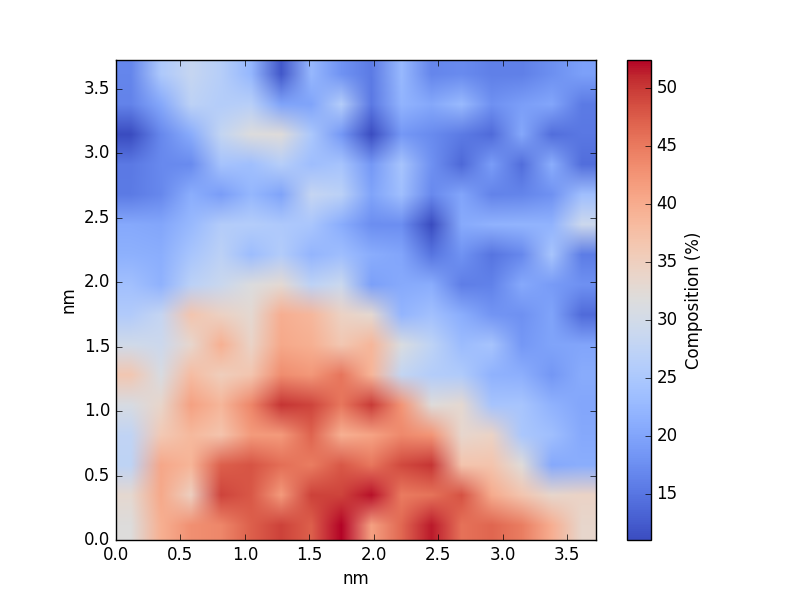
\includegraphics[width=\textwidth]{fig/q/D_heated/_binned_Ge_zetaAbs}
		\caption{Ge}
		\label{fig:Dge}
	\end{subfigure}%
	\hfill
	\begin{subfigure}{0.45\textwidth}
		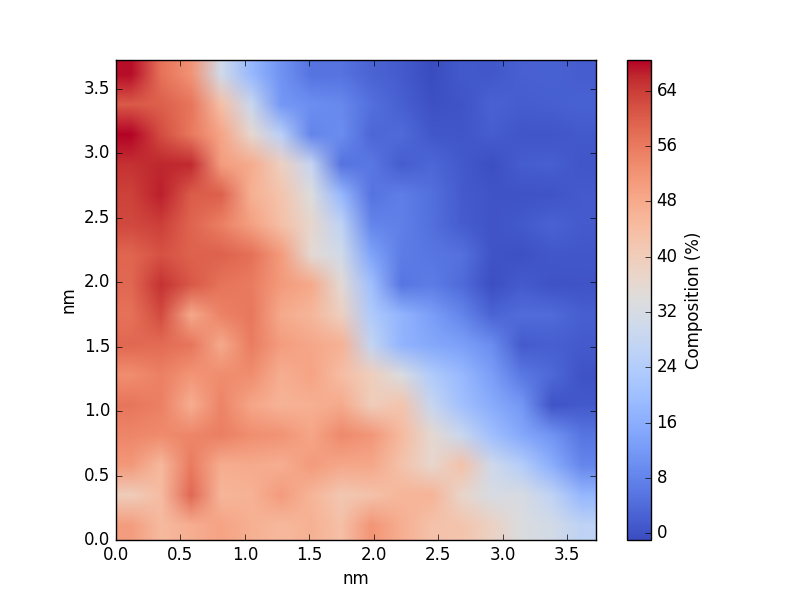
\includegraphics[width=\textwidth]{fig/q/D_heated/_binned_Pd_zetaAbs}
		\caption{Pd}
		\label{fig:Dpd}
	\end{subfigure}
	\caption{plots of....}
	\label{fig:D}
\end{figure}

\begin{figure}
	\centering
	\begin{subfigure}{0.45\textwidth}
		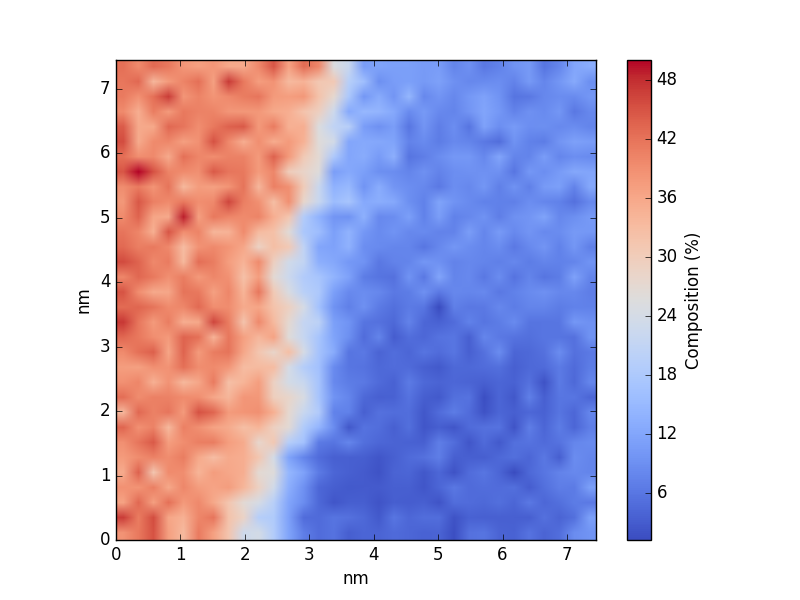
\includegraphics[width=\textwidth]{fig/q/E_heated/_binned_As_zetaAbs}
		\caption{}
		\label{fig:Eas}
	\end{subfigure}%
	\hfill
	\begin{subfigure}{0.45\textwidth}
		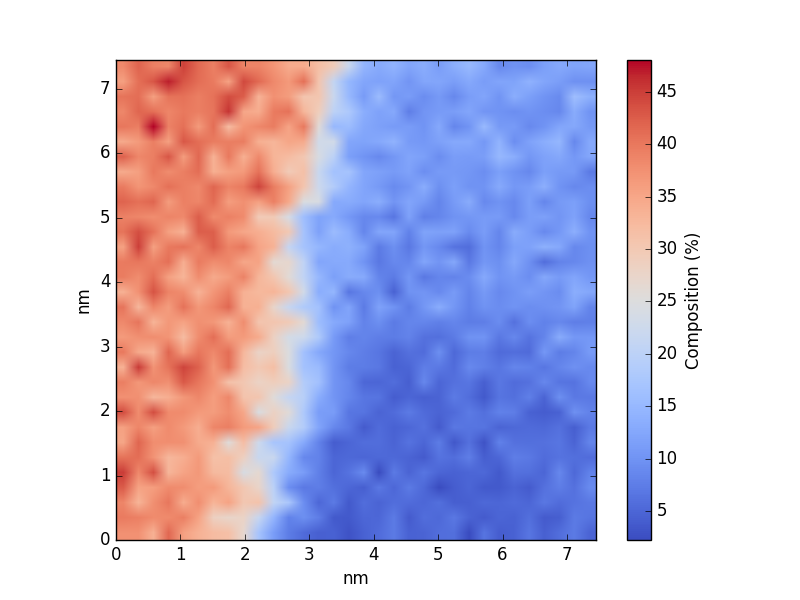
\includegraphics[width=\textwidth]{fig/q/E_heated/_binned_Ga_zetaAbs}
		\caption{}
		\label{fig:Ega}
	\end{subfigure}
	\centering
	\begin{subfigure}{0.45\textwidth}
		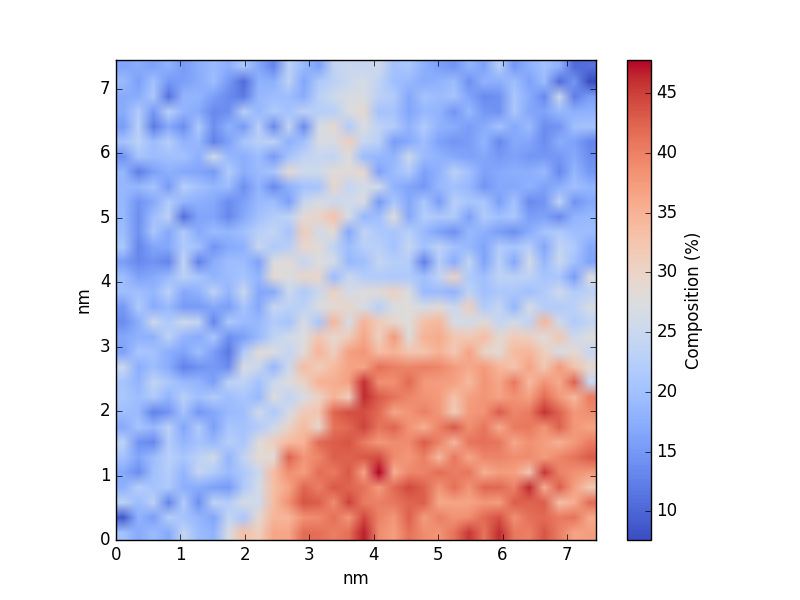
\includegraphics[width=\textwidth]{fig/q/E_heated/_binned_Ge_zetaAbs}
		\caption{}
		\label{fig:Ege}
	\end{subfigure}%
	\hfill
	\begin{subfigure}{0.45\textwidth}
		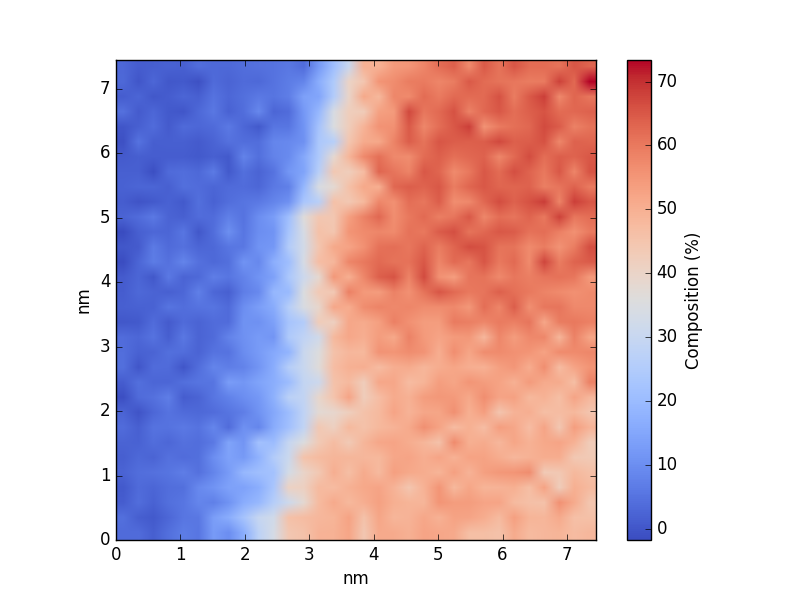
\includegraphics[width=\textwidth]{fig/q/E_heated/_binned_Pd_zetaAbs}
		\caption{}
		\label{fig:Epd}
	\end{subfigure}
	\caption{plots of....}
	\label{fig:E}
\end{figure}

\begin{figure}
	\centering
	\begin{subfigure}{0.45\textwidth}
		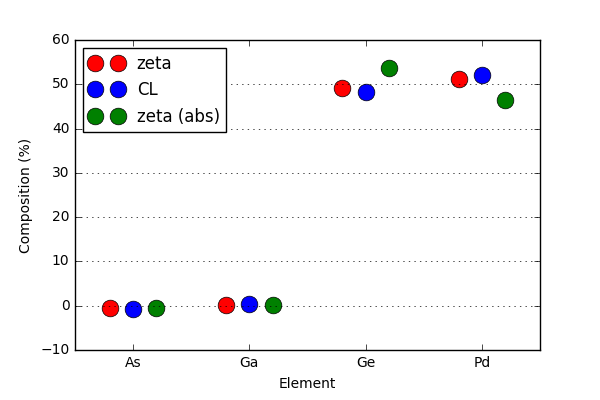
\includegraphics[width=\textwidth]{fig/q/B-C-F/B2}
		\caption{}
		\label{fig:BCF-plots-B}
	\end{subfigure}
	\hfill
	\begin{subfigure}{0.45\textwidth}
		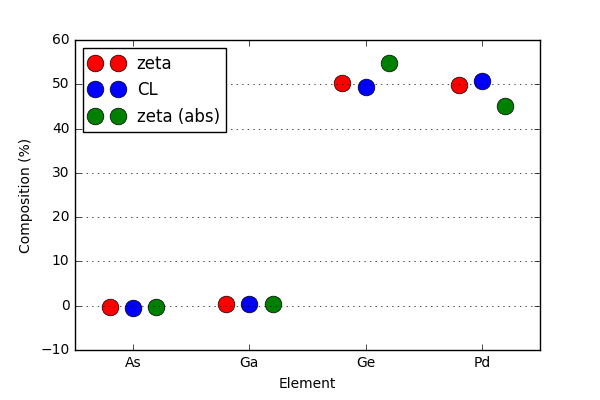
\includegraphics[width=\textwidth]{fig/q/B-C-F/C2}
		\caption{}
		\label{fig:BCF-plots-C}
	\end{subfigure}
	\begin{subfigure}{0.45\textwidth}
	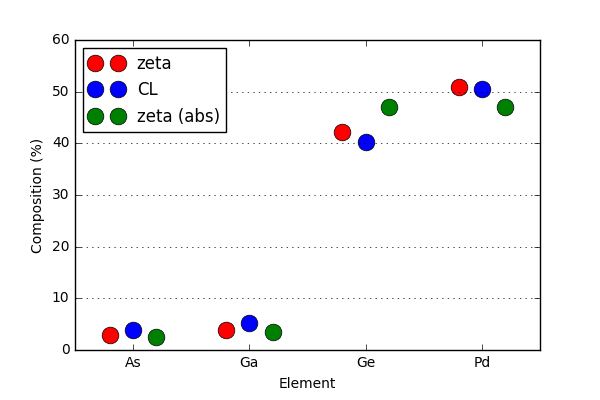
\includegraphics[width=\textwidth]{fig/q/B-C-F/F2}
	\caption{}
	\label{fig:BCF-plots-F}
\end{subfigure}
\hfill
\begin{subfigure}{0.45\textwidth}
	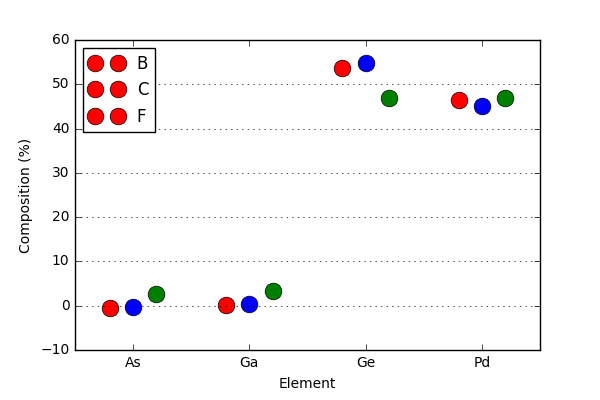
\includegraphics[width=\textwidth]{fig/q/B-C-F/all}
	\caption{}
	\label{fig:BCF-plots-all}
\end{subfigure}
	\caption{
		\label{fig:BCF-plots}%
		Caption}
\end{figure}


Other results:
Angle went from -92.2411 to -94.8174790902
Scale was modified by a factor 0.925757575758
